\section{本章小结}
\label{sec:dcomp-summary}

章首的问题是：两份概率表$P=(0.6,0.3,0.1)$与$Q=(0.3,0.3,0.4)$差多少。本章的回答是，先问差别会在哪里造成后果，再选比较量。表~\ref{tab:dcomp-summary-example}把例表上算出的各个量放在一起。

\begin{BookInlineTable}
 \centering
 \caption{例表上的各比较量（自然对数；MMD用$\sigma=1$的高斯核）。}
 \label{tab:dcomp-summary-example}
 \begin{tabular}{lll}
  \toprule
  比较量 & 数值 & 回答的问题\\
  \midrule
  $d_{\mathrm{TV}}$ & $0.3$ & 同一事件的概率最多差多少\\
  $D_{\mathrm{KL}}(P\Vert Q)$，$D_{\mathrm{KL}}(Q\Vert P)$ & $0.2773$，$0.3466$ & 平均对数比，方向不同\\
  $d_{\mathrm{H}}$，$B$ & $0.2752$，$0.9243$ & 平方根密度的弦长与重叠\\
  $D_{\mathrm{JS}}$ & $0.0737$ & 相对平均分布的KL，有界\\
  $D_{1/2}$，$D_{2}$ & $0.1575$，$0.4220$ & 不同幂次加权的对数比\\
  $\operatorname{MMD}_k$ & $0.3945$ & 核均值之差\\
  $W_1$，$W_2$ & $0.6$，$0.7746$ & 搬运质量的最小成本\\
  \bottomrule
 \end{tabular}
\end{BookInlineTable}

四个角度各有所长。总变差控制所有事件与有界函数，不需要底层距离，但对微小平移与相互奇异的分布一律给出最大值。密度比较量在同一支配测度下比较同一位置的权重：KL散度有似然比的含义并且不对称，Hellinger距离是平方根密度之间的真正距离，JS散度借助平均分布保持有限，Rényi散度用阶数调节对大比值的敏感程度；它们中的$f$散度都满足后处理不增的性质。积分概率度量由测试函数类决定能看见什么，核均值把RKHS单位球上的上确界变成两个核均值之差的范数。Wasserstein距离保留底层几何，一阶时又是Lipschitz函数上的积分概率度量。

用于控制期望时，要先判断评价函数$g$的类型：有界函数配总变差，Lipschitz函数配$W_1$，RKHS中的函数配MMD；无界函数必须把尾部单独拿出来，用一致可积或高阶矩控制；用KL散度控制期望时，需要参考分布下的指数矩，并且方向要与散度的参数对应。

用于收敛时，各比较量之间的关系汇总在图~\ref{fig:dcomp-implication-map}中。KL散度通过Pinsker不等式控制总变差，总变差与Hellinger距离相互控制，总变差收敛推出弱收敛而反之不然；$W_p$收敛等于弱收敛加$p$阶矩收敛；$\mathbb{R}^{d}$上固定带宽的高斯核MMD收敛恰好等于弱收敛。反过来的每一个缺口都有反例：零概率格点使小总变差对应无穷KL，单点平移与格点逼近使弱收敛不带来总变差收敛，远处的小质量使弱收敛与MMD收敛不带来矩的收敛，不连续的特征核使MMD不再刻画弱收敛。

\begin{BookInlineFigure}
 \centering
 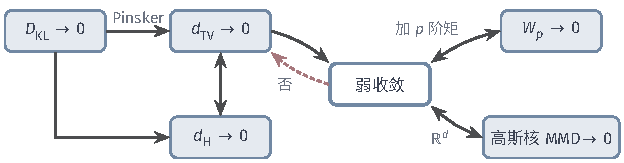
\includegraphics[width=106mm]{figures/07-probability/04-distribution-analysis/tikz/dcomp-implication-map/figure.pdf}
 \caption{本章证明或引用的收敛关系，均指$P_n$与固定的$P$之间的比较量趋于零。实线箭头表示蕴含，双向箭头表示等价（$W_p$需加上$p$阶矩收敛，高斯核MMD限于$\mathbb{R}^{d}$），红色虚线表示反向不成立。}
 \label{fig:dcomp-implication-map}
\end{BookInlineFigure}

第~\ref{chap:distribution-approximation}章在限定的候选族中寻找与目标最接近的分布时，就要用这里的比较量衡量误差，并按任务选择方向。第~\ref{chap:dependence-measures}章把联合分布与边缘乘积作比较，用KL散度得到互信息，用MMD得到HSIC。从有限样本估计这些比较量、评价估计误差并据此检验两个分布是否相同，属于卷八的内容。
